\documentclass[]{article}

\usepackage{graphicx}

%opening
\title{ARTS1422 HW1}
\author{Suting Chen}

\begin{document}

\maketitle

\section{Requirements}
All code has been tested on Chrome and Safari only. They are guaranteed to work with D3.js.v5

\section{Task 1}
Press the problem 1 button below to show the first figure: 
\begin{center}
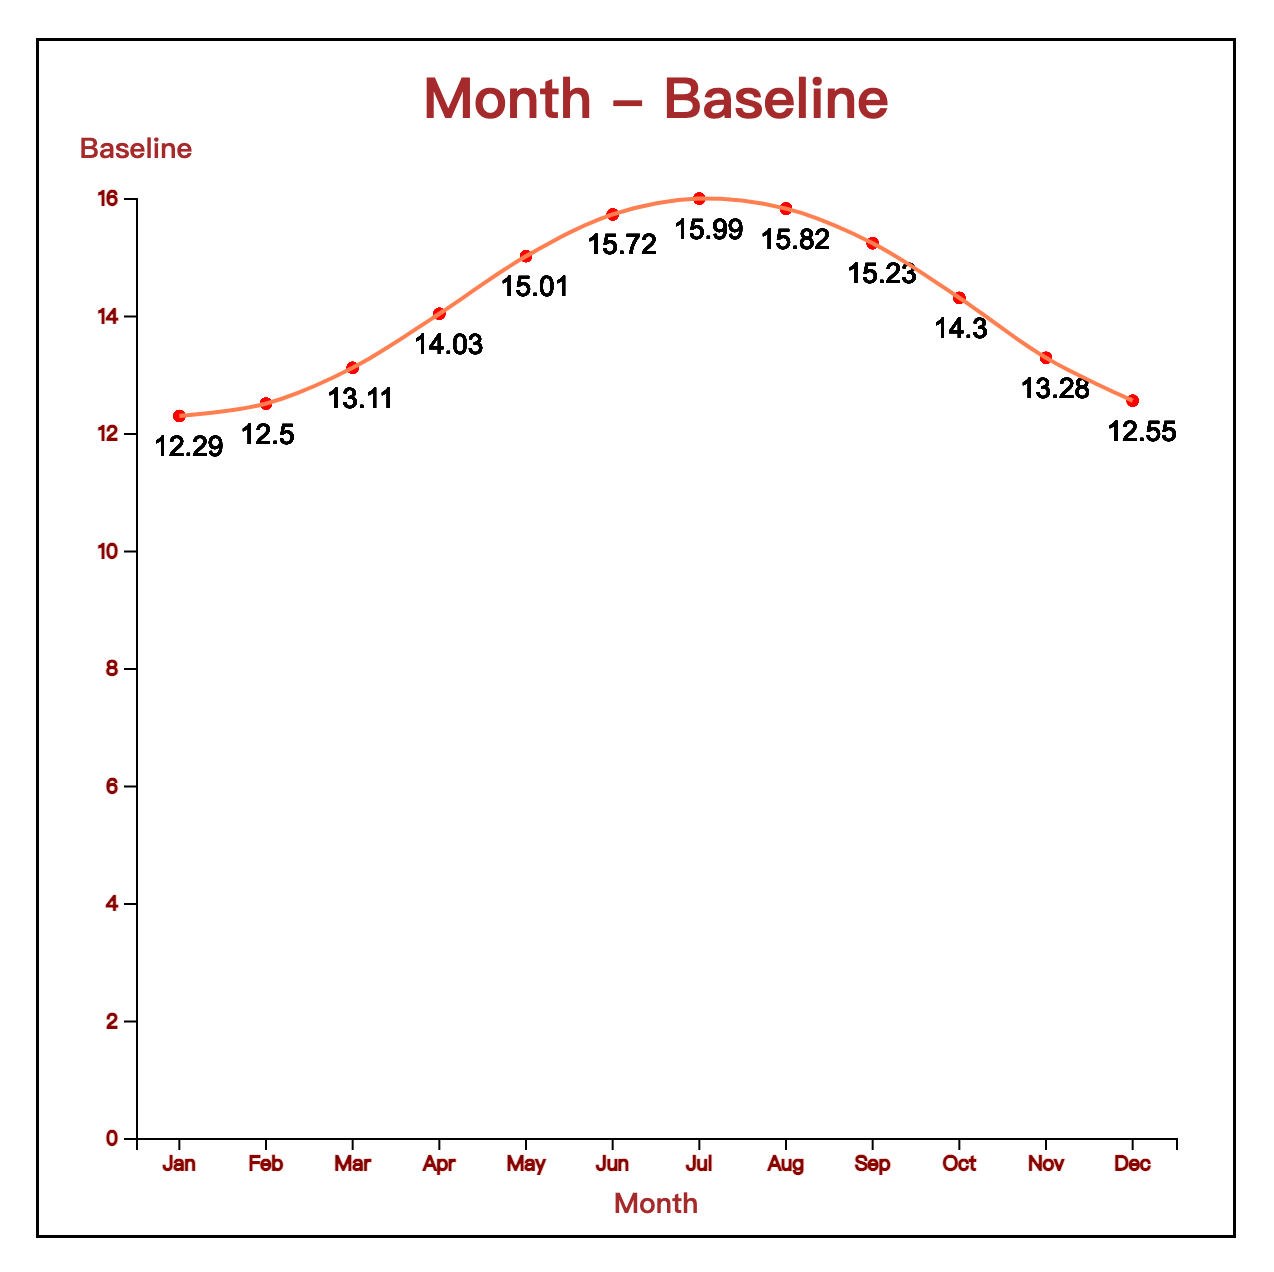
\includegraphics[width=0.7\linewidth]{task1}
\end{center}
Here we have name of months as X axis, value of baselines as Y axis.

\newpage

\section{Task 2}
Press the problem 2 button below to show the second figure: 
\begin{center}
	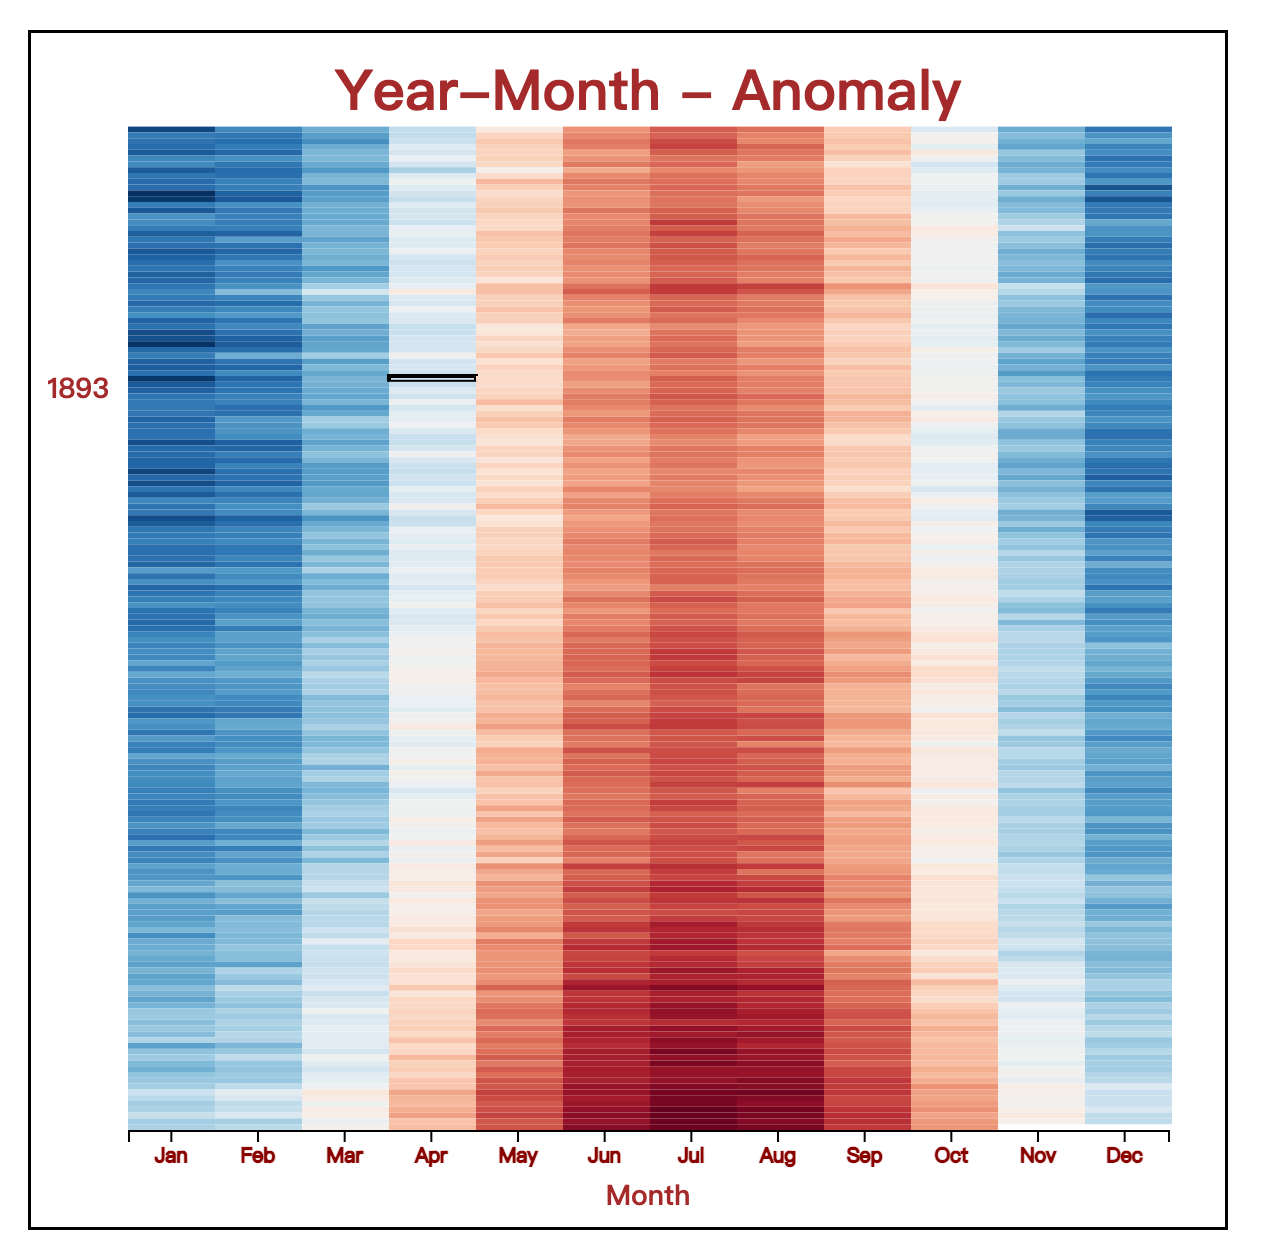
\includegraphics[width=0.7\linewidth]{task2}
\end{center}
Visualization of data in the .csv file is achieved by normalizing and harnessing $d3.interpolateRdBu$.

We can easily find out that, as time goes by, temperature gradually rises.



\end{document}
